\chapter{研究背景}
\label{chap:webapi}

本章では本研究の背景を、ユーザーの拡張現実や明晰夢における認識度や要求について事前調査・分析をし、それに基づいてDreamScapeの開発に反映した点について述べる。

\section{拡張現実について調査}
理系の学生7人、文系の学生7人、サラリーマン10人、主婦3人を含めた20〜60歳の男女27人に対するインタビューをから、それぞれがどのような拡張現実を望んでいるかを調査するためにオンラインアンケートを集めた。これらのインタビュー結果を経て一般的なユーザのニーズを把握し、DreamScapeの有効性やDreamScapeが解決すべき問題について明らかにする。

\subsection{拡張現実を体験するために一般的な人々が支払う金額}
機能性やデザインの詳細を説明した上で、仮想現実を見る手段として次の選択肢から選んでもらった。OCULOUS Rift:85278円、ハコスコ:1500円、iWink:36478円、タカラトミー夢工房:15984円、DreamScape :無料。すると図\ref{userNeedCost}のように、一般的なユーザーの中には拡張現実を体験するためにOCULOUS Riftなどの高額なデバイスを購入しようとする人は少ないということが分かった。ハコスコだと少し数が増えるが、これらのデータから無料で簡単に手に入れることができるツールを多くの人が必要としていることが証明された。

\begin{figure}[htbp]
\begin{center}
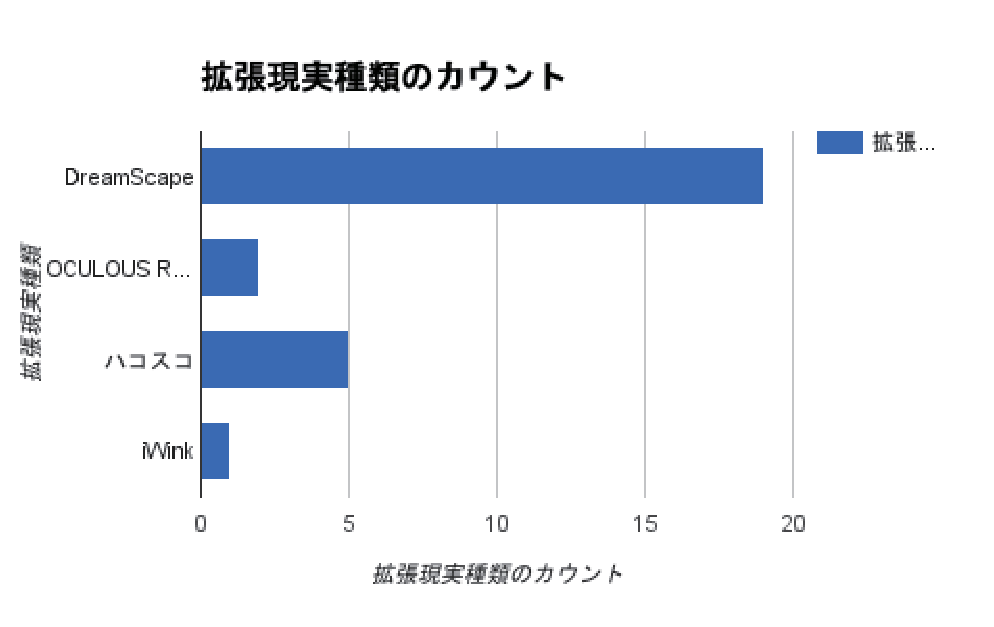
\includegraphics[width=15cm]{eps/VRselection.eps}
\caption{拡張現実を体験するために一般的ユーザーが選ぶ手段}
 \label{userNeedCost}
\end{center}
\end{figure}

\subsection{拡張現実を体験したいタイミング}
拡張現実を体験したいタイミングとして、睡眠中と起きている時間帯でどちらが好ましいかについて調査を行った。すると図\ref{VRtiming}のようにあまり差がなかった。睡眠中を選択した人は理由として「睡眠時間の有効活用のため」と答えた。比べて起きている時と選択した人は「起きたら忘れてしまうかもしれないから、意識のある時に体験したい」と答えた。よってDreamScapeの開発において実際に睡眠中の拡張現実がユーザーにどのような体験を与えるかを研究することは意義があると考えられる。

\begin{figure}[htbp]
\begin{center}
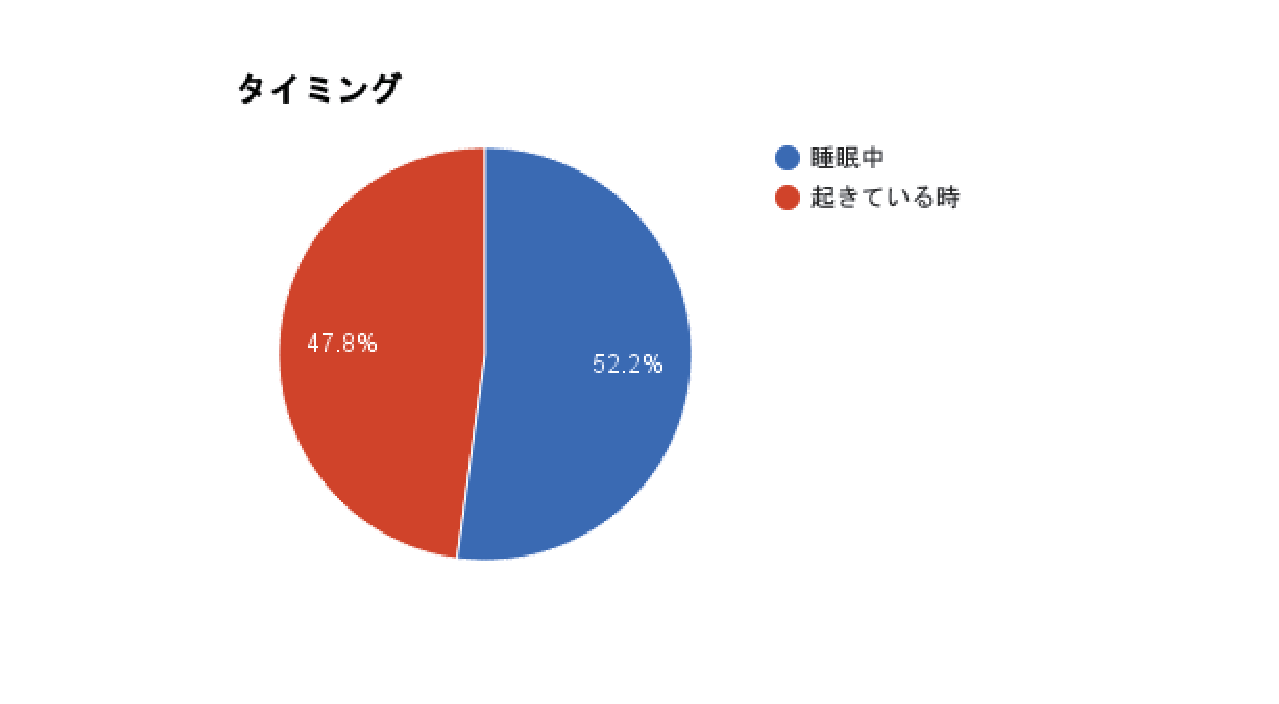
\includegraphics[width=15cm]{eps/timing.eps}
\caption{拡張現実を体験したいタイミング}
\label{VRtiming}
\end{center}
\end{figure}

\section{明晰夢に関する調査}
\subsection{夢をどのくらい記憶しているか}
夢の操作に成功したとしてもその夢を覚えていなければ意味がない。そこで実験を始める前に一般的に人は夢の内容を起床後どのくらい覚えているのかを調査した。図\ref{rememberDream}がから読み取れるように、夢をよく覚えていると答えた人は少数だった。

\begin{figure}[htbp]
\begin{center}
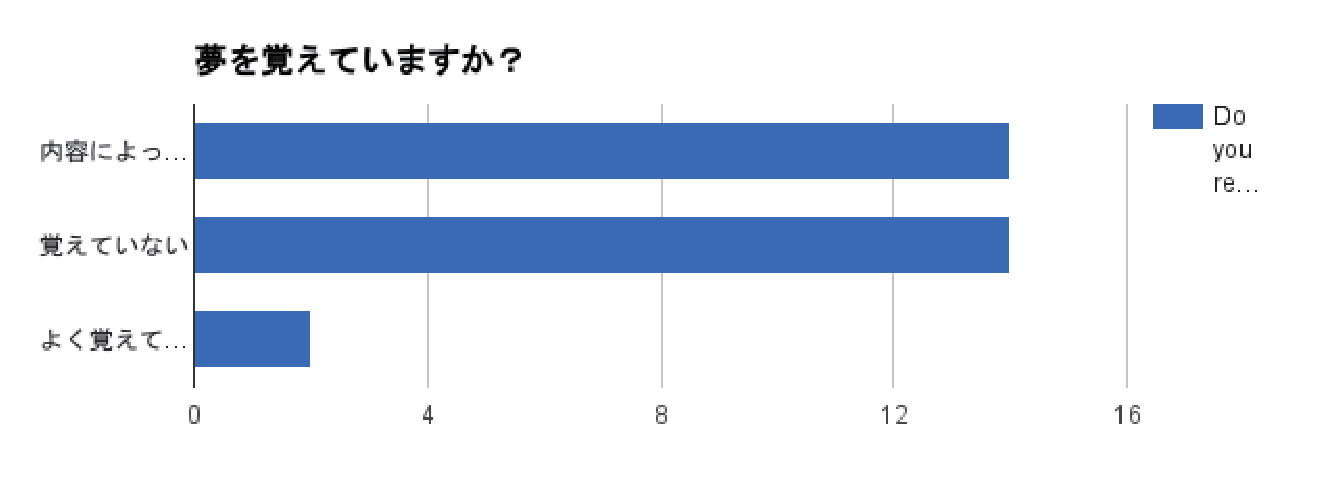
\includegraphics[width=15cm]{eps/remember.eps}
\caption{夢を覚えている比率}
\label{rememberDream}
\end{center}
\end{figure}

覚えている夢は刺激的、怖い夢、繰り返し見た夢というのが多く、日常的な夢は忘れがちであるということが分かった。人は睡眠中5回ほど夢を見ていると言われているがその90\%を起床後5分間で忘れるという。夢を忘れないためによく取られる手法は夢日記である\cite{forgetDreams}。よってDreamScapeには5分以内に夢の内容を記憶するための日記の機能を加えることに決めた。夢日記は習慣的につけることで効果が出ると言われている。この事実からDreamScapeの被験者には2週間前から枕の横に紙とペンを置いて起床後すぐに夢の内容を書く習慣を付けてもらうことにした。

\subsection{夢に影響を与えやすい外的刺激}
心理学者フロイトは「夢判断」の中で人は睡眠中の姿勢、環境、身体的刺激によって夢の内容が変化すると述べている\cite{freud}。睡眠中の人間の鼻先を羽毛でくすぐったときに、夢の内容に変化があったことを確認する実験を紹介している。そこで音、体制、匂い、振動、光、などの刺激の中で何が夢に一番影響を与えやすいのかの調査をした。以下の図\ref{externalShigeki}がその結果を示す。音が他の刺激よりも影響を与えやすいということが分かった。DreamScapeにとって刺激は非常に重要な鍵となるので実験を通してどの刺激が最も有効的なのかを調べた。それについて第3章を参照してほしい。

\begin{figure}[htbp]
\begin{center}
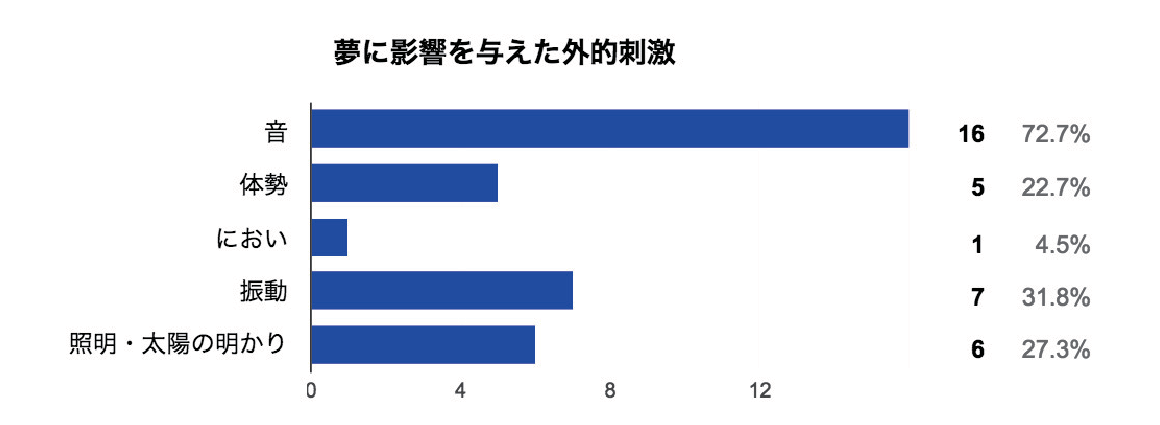
\includegraphics[width=15cm]{eps/input.eps}
\caption{夢に影響を与えた外的刺激}
\label{externalShigeki}
\end{center}
\end{figure}

\subsection{明晰夢のニーズ}
明晰夢を体験したいか否かで質問をしたところ、図\ref{lucidNeeds}からも分かるように77\%の人が体験したいと答えた。よってDreamScapeのニーズもあると仮定する。
\begin{figure}[htbp]
\begin{center}
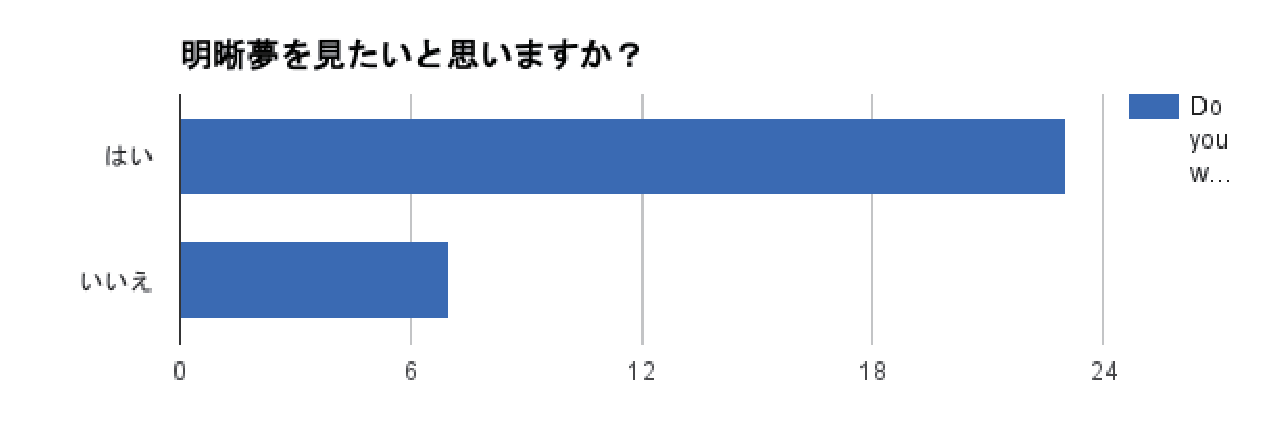
\includegraphics[width=15cm]{eps/lucidDreamingYesNo.eps}
\caption{明晰夢のニーズ}
\label{lucidNeeds}
\end{center}
\end{figure}

\subsection{明晰夢で体験したい内容}
拡張現実で体験したい内容を調査結果から似ているものをカテゴリー別に分けて、図\ref{desiredDreamTpye}で示した。LOVEタイプ、癒し、元気欲しいタイプ、アドベンチャータイプ、ストーリータイプ、ビジネスタイプとあるがそれぞれの定義を述べる。LOVEタイプとは恋愛や性的行為などが含まれる内容。アドベンチャータイプは冒険など非日常の体験を求める内容。ストリータイプはドラマのように連続性のある夢を求める内容。癒しタイプ・元気欲しいタイプは娯楽を求める内容。原強化タイプは睡眠中になんらかの学習を求める内容だ。LOVEタイプと癒し・元気が欲しいタイプが最も多く、少数派として勉強家タイプがあった。

\begin{figure}[htbp]
\begin{center}
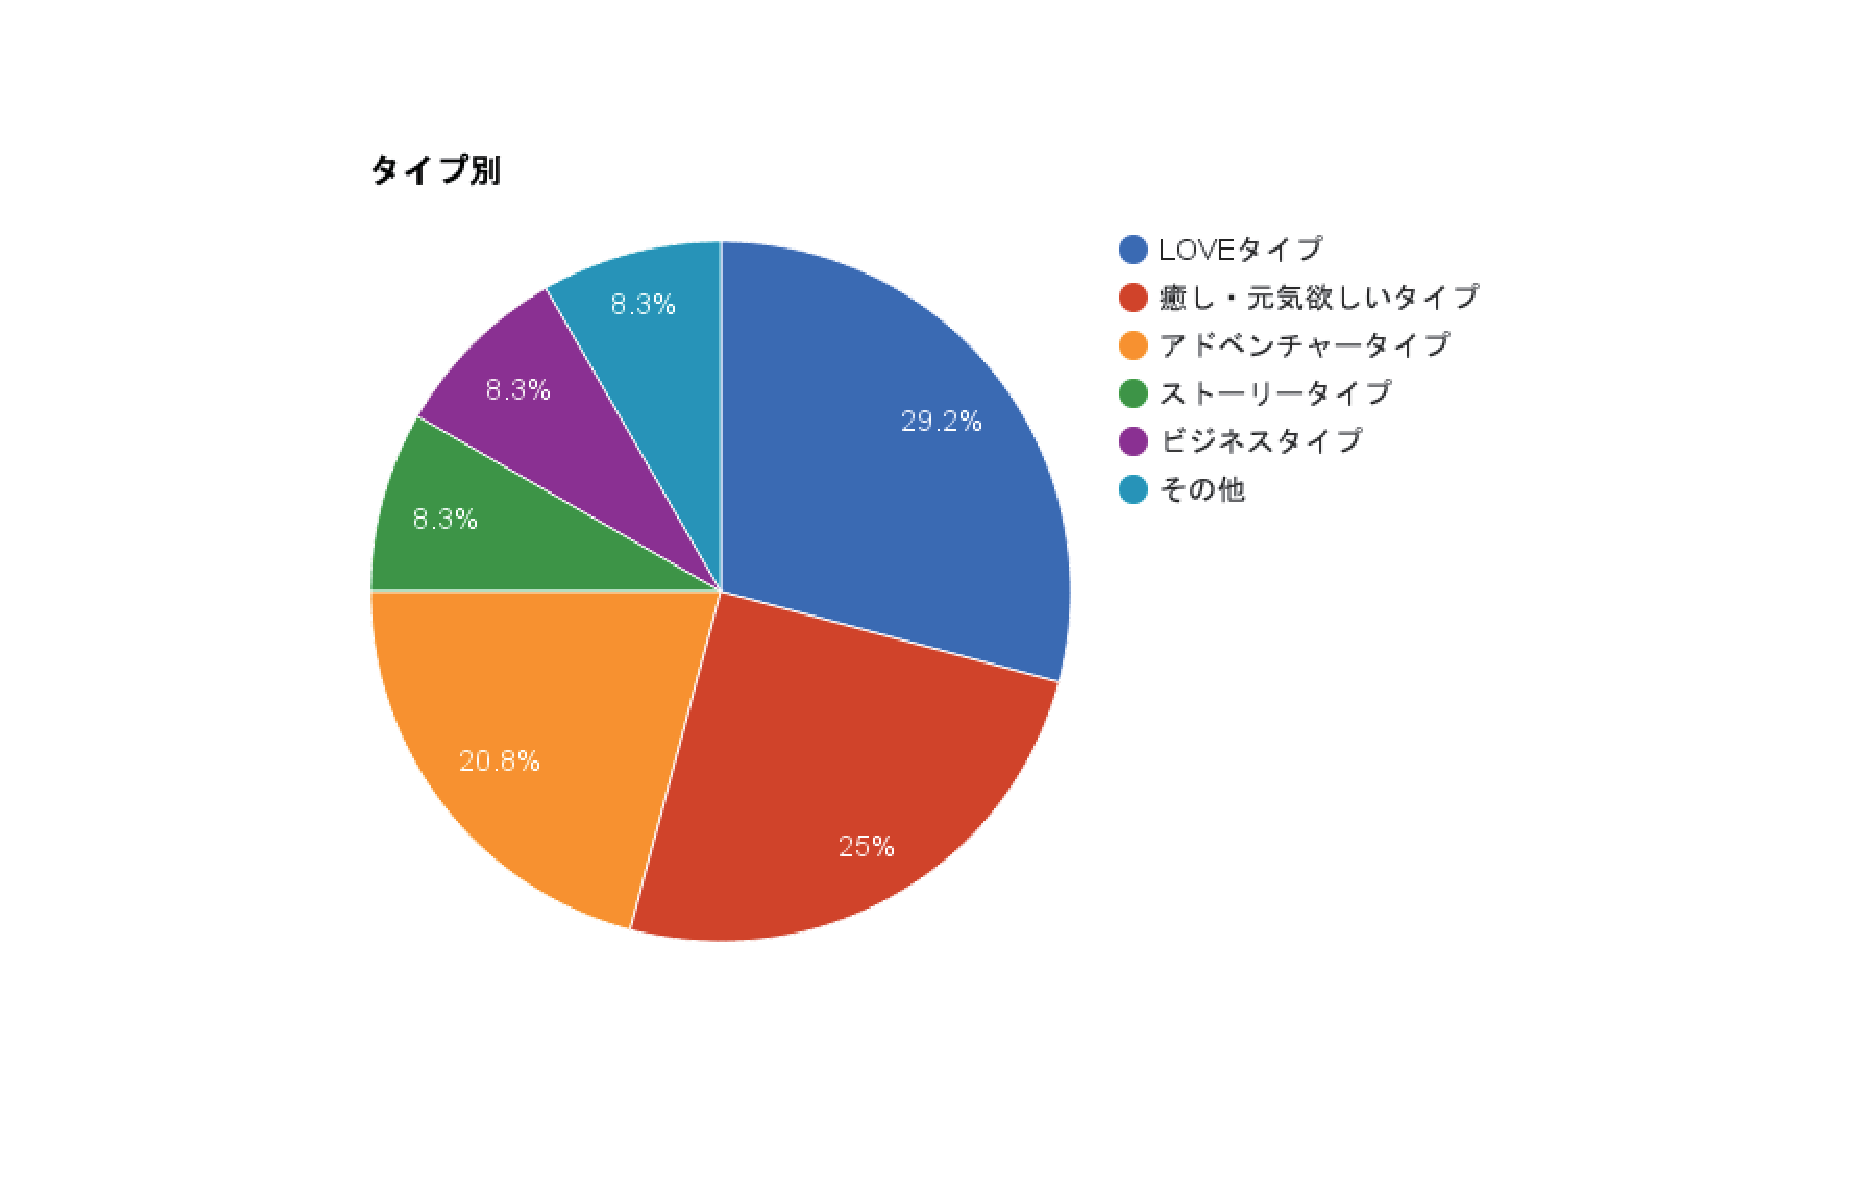
\includegraphics[width=15cm]{eps/dreamType.eps}
\caption{明晰夢で体験したい内容:分析1}
\label{desiredDreamTpye}
\end{center}
\end{figure}

回答をさらに違った方法で分析した結果が\ref{desiredDreamTpye2}である。これらの結果から、ユーザーの求める夢体験を把握することができたので、DreamScapeの目標をこれらの夢の実現とする。

\begin{figure}[htbp]
\begin{center}
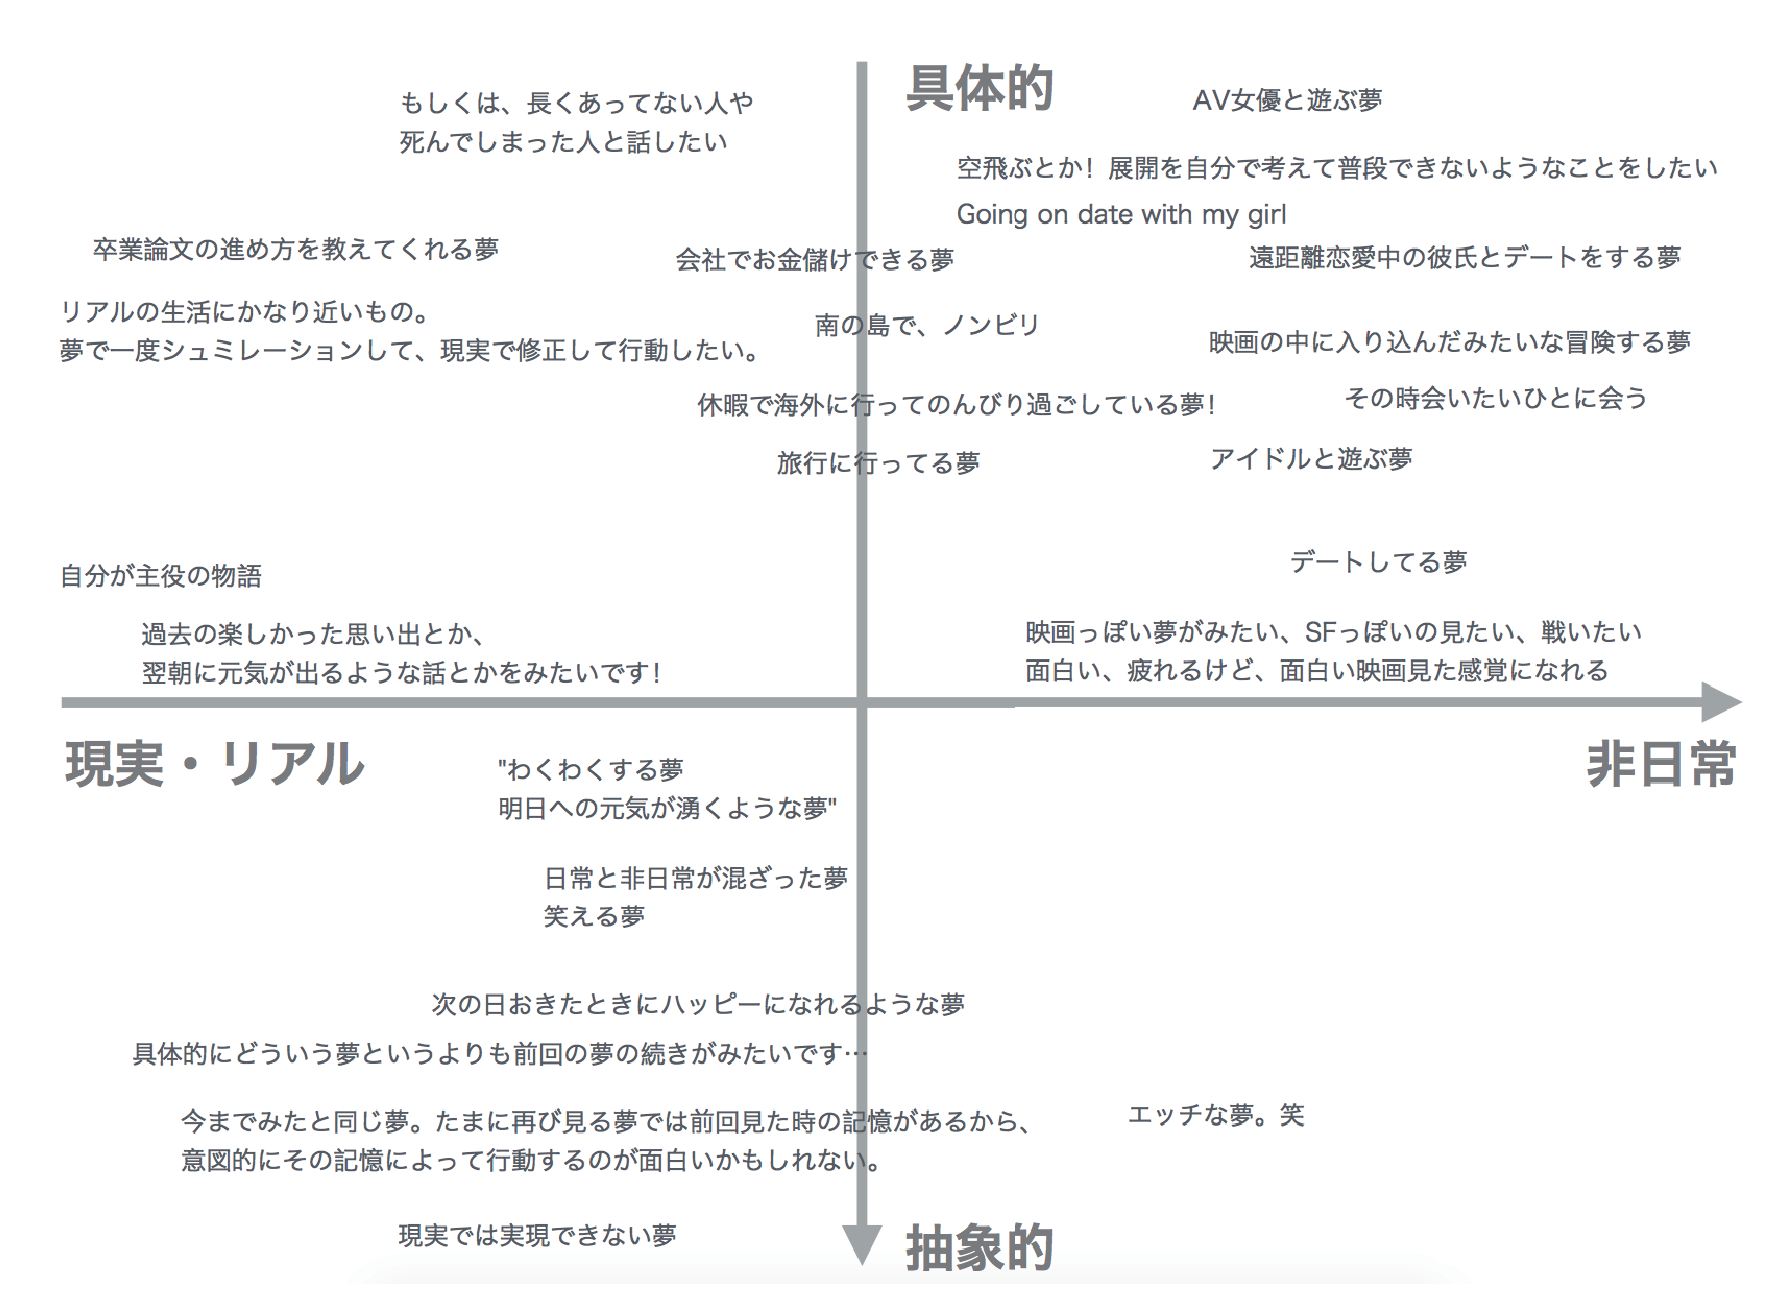
\includegraphics[width=15cm]{eps/whatYouWantToDream.eps}
\caption{明晰夢で体験したい内容:分析2}
\label{desiredDreamTpye2}
\end{center}
\end{figure}

\section{調査から分かったこと}
現実を仮想的に見ることが明晰夢でも可能なのであれば、DreamScapeにも興味を示す人が多いということが分かった。明晰夢は睡眠という習慣をより有効に活用し、金銭的コストをかけることなく遂行することができる。求められるのは低価格、高機能、快適なユーザー体験なのでその点に気をつけて開発を進めたい。またコンテンツが見られるようにする対策も必要であろう。